\documentclass[twoside,11pt]{article}

% Any additional packages needed should be included after jmlr2e.
% Note that jmlr2e.sty includes epsfig, amssymb, natbib and graphicx,
% and defines many common macros, such as 'proof' and 'example'.
%
% It also sets the bibliographystyle to plainnat; for more information on
% natbib citation styles, see the natbib documentation, a copy of which
% is archived at http://www.jmlr.org/format/natbib.pdf

% Available options for package jmlr2e are:
%
%   - abbrvbib : use abbrvnat for the bibliography style
%   - nohyperref : do not load the hyperref package
%   - preprint : remove JMLR specific information from the template,
%         useful for example for posting to preprint servers.
%
% Example of using the package with custom options:
%
%\usepackage[abbrvbib, preprint]{jmlr2e}
\usepackage{jmlr2e}
\usepackage{booktabs}
\usepackage{hyperref}
\usepackage{amsmath}

\usepackage{graphicx}
\usepackage{subcaption}

% Definitions of handy macros can go here
\newcommand{\dataset}{{\cal D}}
\newcommand{\fracpartial}[2]{\frac{\partial #1}{\partial  #2}}
\usepackage{xcolor}
\definecolor{diffcolor}{rgb}{0.16, 0.32, 0.75}
\newcommand{\diff}[1]{\textcolor{diffcolor}{#1}}

% Heading arguments are {volume}{year}{pages}{date submitted}{date published}{paper id}{author-full-names}
\usepackage{lastpage}
\jmlrheading{}{2022}{1-\pageref{LastPage}}{}{}{}{}

% Short headings should be running head and authors last names
\ShortHeadings{Mixture of Experts for Tokenformer}{Khodzina, Kozakiewicz, Misiaszek, Znamierowski}
\firstpageno{1}

\begin{document}

\title{Mixture of Experts for Tokenformer
}

\author{\name Anastasiya Khodzina \email a.khodzina@student.uw.edu.pl \\
    \name Ignacy Kozakiewicz \email ik448298@students.mimuw.edu.pl \\
    \name Jakub Misiaszek \email jm448365@students.mimuw.edu.pl \\
    \name Mikołaj Znamierowski \email mz430283@students.mimuw.edu.pl \\
    \addr University of Warsaw, Poland\\
}

\maketitle







%==========================================================

\begin{abstract}%
Recent developments in NLP have lead to multiple proposals for modifications of the Transformer architecture. Two of them - Tokenformer and Mixtral of Experts - aim to increase respectively the scalability and the accuracy of the models. In this work we propose to combine these two ideas into one architecture, and compare its performance on two different benchmarks. What we discover is that these ideas work well together, and achieve high performance, while keeping the scalability mechanisms intact.
\end{abstract}






\section{Introduction}

Transformers \cite{Attention_is_all_you_need} have become the dominant architecture in the field of Natural Language Processing (as well as many other domains), achieving state-of-the-art results. Their computations on a single token are of two distinct types: interactions with other tokens, and with the model parameters. While the first are facilitated by the attention mechanism, which scales greatly, the second type relies heavily on linear projections. This design limits scalability, as size-altering introduces architectural differences, which usually requires retraining the model from scratch (as shown in \cite{Scaling}).

This issue has been addressed recently in \cite{Tokenformer}. The paper proposes to modify the transformer's architecture (achieving, what they call, a \textit{Tokenformer}) by replacing all standard linear projections with new \textit{pattention} layers, and treating the model's parameters as tokens, applying a modified attention mechanism on them. This approach significantly improves scalability, while achieving comparable accuracy.

On the other hand, Mixtral of Experts - another modification of the transformer architecture - arose in \cite{MoE}. The goal is to improve the model's performance by replacing the standard FFN layers with multiple Experts, each processing different sets of tokens (which is decided and weighted by the Router before the Experts).

In this work, we aimed to answer the following question: can these two changes work together? If so, this might give rise to a new type of transformers, that is both accurate and easily scalable. We discovered that the answer is yes - based on the main results in table \ref{tab:results}, we can safely say that the performance of this combination of architectures is as good as the plain Transformer with MoE, while keeping the same scaling ability as Tokenformer.









\section{Methodology}

We combined two architectural modifications of transformers: use MoE instead of FFNs, and, on top of that, replace all linear projections with pattention layers. To be more precise:

\subsection{MoE}

We want the input tokens to only be processed by appropriate Experts (FFNs with different weights instead of one FFN for all the tokens), so that the model can get specialized on several fields, without the loss of compute. A graphical representation is shown in figure \ref{fig:orig_MoE}. Formaly, MoE algorithm can be summarized in the following way:

Suppose we have $n$ Experts $\{E_1, E_2, \ldots, E_n\}$ and an input $x$. Then, the output of MoE is calculated as
$$\sum_{i=1}^n G(x)_i \cdot E_i(x)$$
Here, $G(x)_i$ denotes the $n$-dimensional output of the gating network (the Router) for the $i$-th Expert, and $E_i(x)$ is the output of the $i$-th Expert network. More specifically, we use
$$G(x) = \text{Softmax}(\text{TopK}(x \cdot W_g))$$
Where $W_g$ is the gating matrix (the Router), and $\text{TopK}(l)_i = l_i$ if $l_i$ is among the top-K coordinates of logits $l \in \mathbb{R}^n$ and $\text{TopK}(l)_i = - \infty$ otherwise.


\begin{figure}[h]
\centering

    \begin{subfigure}{0.6\textwidth}
        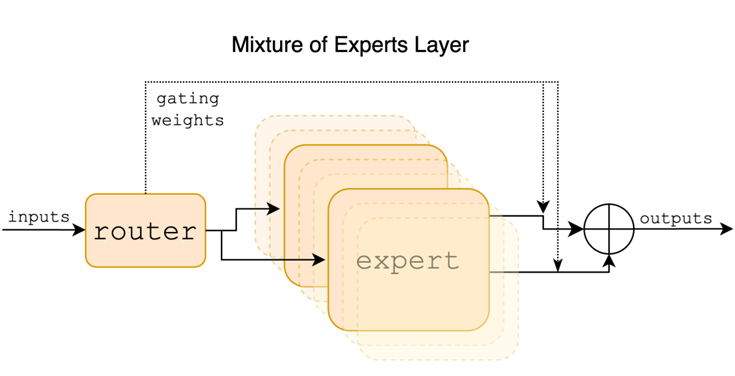
\includegraphics[width=0.95\linewidth]{Figures/moe_podstawowy.png}
        \caption{Original Mixtral of Experts}
        \label{fig:orig_MoE}
    \end{subfigure}
    \begin{subfigure}{0.39\textwidth}
        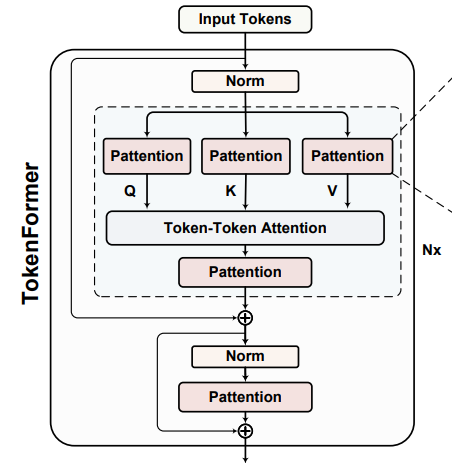
\includegraphics[width=0.95\linewidth]{Figures/tokenformer_podstawowy.png}
        \caption{Original Tokenformer block}
        \label{fig:orig_tokenformer_block}
    \end{subfigure}
        
\caption{Original modifications of the transformer architecture}
        
\end{figure}


\subsection{Pattention layer}

We want to replace each linear projection with the so-called \textit{pattention layer}. Originally, this layer is used as in figure \ref{fig:orig_tokenformer_block}. The idea is to leverage the power of attention not just in the token-token interactions, but also in token-parameter ones. To achieve this, we will treat the model parameters as learnable tokens, and apply a modified attention mechanism on them. The layer can be described as follows:

Suppose we have an input sequence $\mathcal{I} \in \mathbb{R}^{T \times d_1}$ and we want to achieve an output sequence $\mathcal{O} \in \mathbb{R}^{T \times d_2}$, where $T$ is the sequence length, and $d_i$ are the input and output dimensions respectively.

We introduce two sets of $n$ learnable parameter tokens: $K_P \in \mathbb{R}^{n \times d_1}$ representing the keys, and $V_P \in \mathbb{R}^{n \times d_2}$ representing the values. Then, the Pattention is computed as
$$\mathcal{O} = \text{Pattention}(\mathcal{I}, K_P, V_P) = \Theta (\mathcal{I} \cdot K_P^T) \cdot V_P$$
Here, $\Theta$ is a modified softmax operation for stable optimization. More precisely:
\begin{itemize}
    \item Softmax $=$ exp + L1 norm
    \item $\Theta = $ L2 norm + GeLU
\end{itemize}

With this idea, scaling can be done by simply concatenating new parameter tokens (increasing $n$), and learning only those new ones, keeping the old ones frozen.












%\clearpage

\section{Experiments}

We trained four setups:
\begin{itemize}
    \item Transformer without MoE
    \item Transformer with MoE
    \item Tokenformer without MoE
    \item Tokenformer with MoE
\end{itemize}

Both non-MoE-setups had roughly $124$M parameters, while both MoE-setups had roughly $294$M parameters - this ensures a fair comparison inside each class. The training dataset chosen was half OpenWebText and half Pile. We trained all models for $1025$ epochs, and then evaluated the performances on two benchmarks: Pile and HellaSwag. Results can be seen in table \ref{tab:results}. The respective plots can be seen in figure \ref{fig:plots}.

\begin{table}[h]
    \centering
    \begin{tabular}{|c||c c|}
        \hline
        Model \textbackslash Benchmark & Pile perplexity & HellaSwag accuracy \\
        \hline\hline
        Transformer & 15.49 & 0.33 \\
        \hline
        Transformer + MoE & 15.01 & 0.326 \\
        \hline
        Tokenformer & 15.86 & 0.302 \\
        \hline
        Tokenformer + MoE & 14.99 & 0.32 \\
        \hline
    \end{tabular}
    \caption{Comparison of performances of all trained setups on both benchmarks}
    \label{tab:results}
\end{table}

Judging by the results above, the performance of Tokenformer with MoE on both benchmarks is significantly better than that of plain Tokenformer, and comparable with the results of Transformer with MoE. This proves that adding MoE to Tokenformer increases its performance, with no collapse in training. This combination thus gives rise to an architecture that laverages both the power of MoE with the scalability of Tokenformer.

\begin{figure}[h]
\centering
    \begin{subfigure}{0.9\textwidth}
        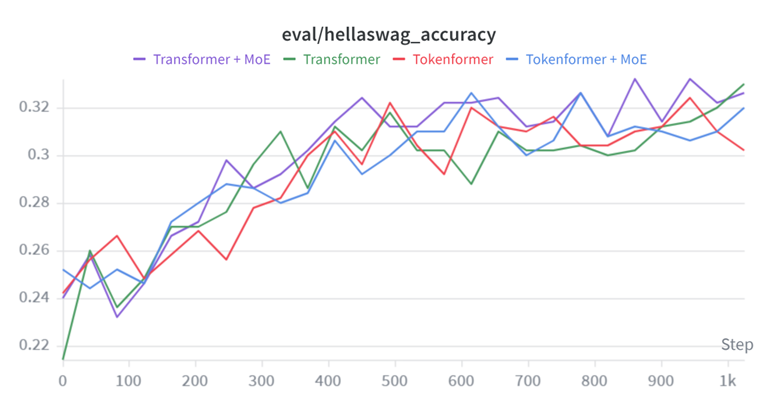
\includegraphics[width=0.95\linewidth]{Figures/hellaswag.png}
        \caption{HellaSwag}
        \label{fig:eval_hellaswag}
    \end{subfigure}
    \begin{subfigure}{0.9\textwidth}
        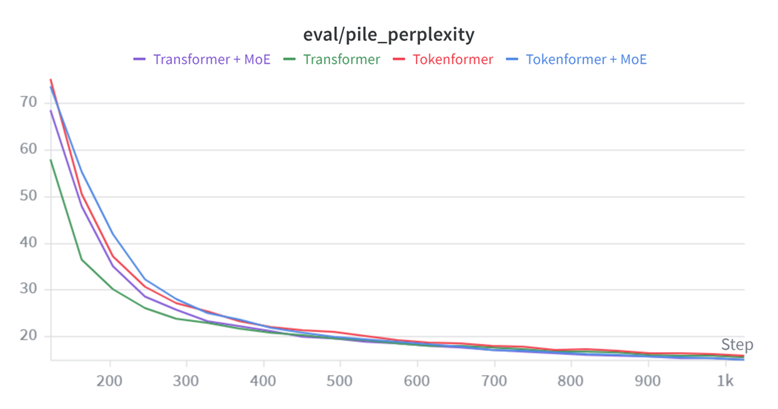
\includegraphics[width=0.95\linewidth]{Figures/pile.png}
        \caption{Pile}
        \label{fig:eval_pile}
    \end{subfigure}
\caption{Main plots comparing all the models on both benchmarks}
\label{fig:plots}
        
\end{figure}








\section{Conclusions}

Previous works have introduced ways of modifying the Transformer architecture, to increase either its performance (Mixtral of Experts, in \cite{MoE}), or scalability (Tokenformer, in \cite{Tokenformer}). In this work we have shown that combining these two ideas doesn't lead to a collapse in learning, and instead gives rise to a new architecture, that has the capacity to be both accurate and scalable. Further works needs to be done to fully optimize the hyperparameters, and the number of training epochs, however, we have shown that those ideas do work together well.








%\nocite{*} % uncomment this if you want to check what your new reference will look like without having to cite it yet
\bibliography{references}









% \clearpage

% \section{Appendix}

% [TODO]




% \begin{figure}[h]
% \centering
%     \begin{subfigure}{0.9\textwidth}
%         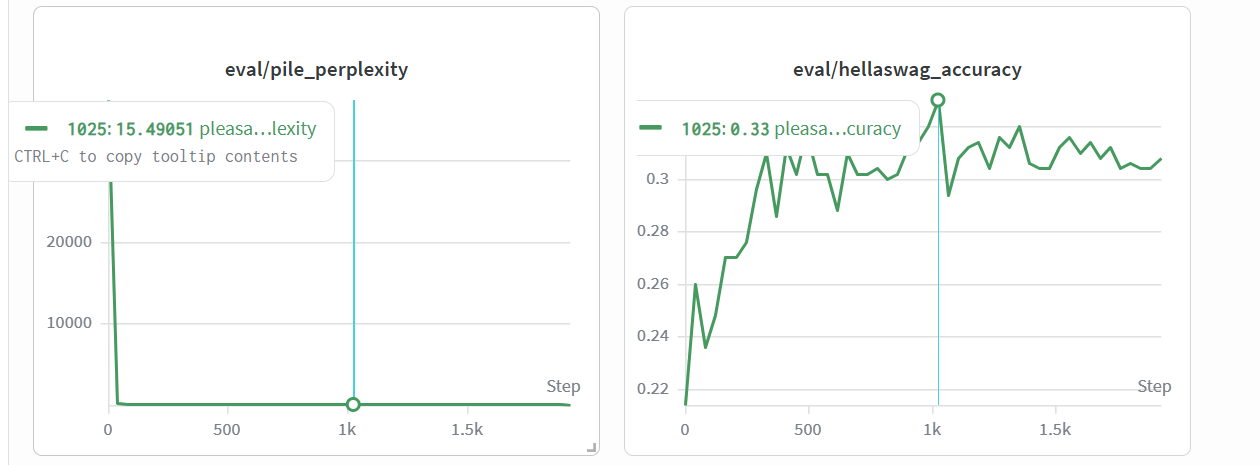
\includegraphics[width=0.95\linewidth]{Figures/transformer_perplexity_hellaswag_1025.png}
%         \caption{Transformer}
%         \label{fig:eval_transformer}
%     \end{subfigure}
%     \begin{subfigure}{0.9\textwidth}
%         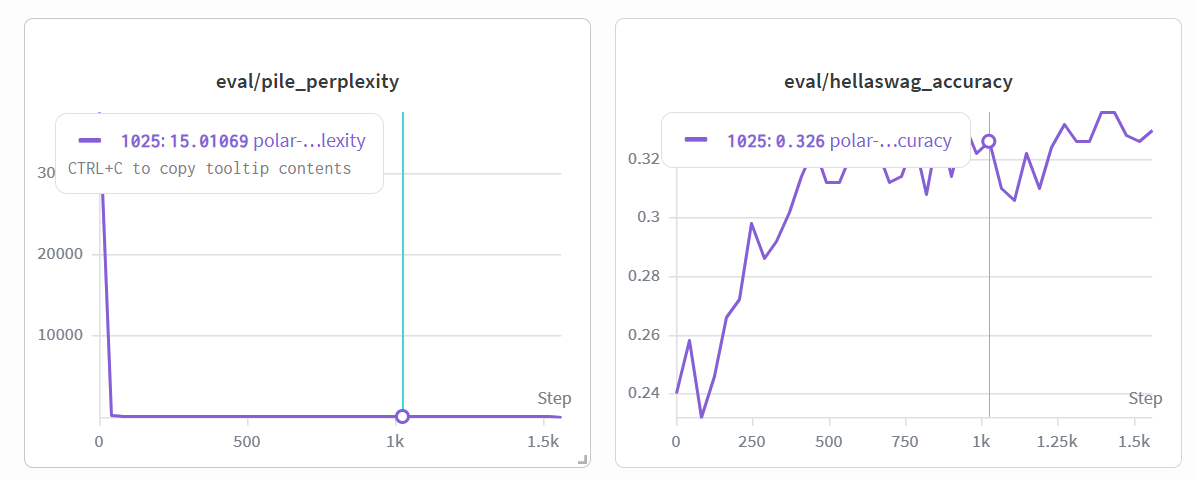
\includegraphics[width=0.95\linewidth]{Figures/transformer_moe_perplexity_hellaswag_1025.png}
%         \caption{Transformer + MoE}
%         \label{fig:eval_transformer_moe}
%     \end{subfigure}
%     \begin{subfigure}{0.9\textwidth}
%         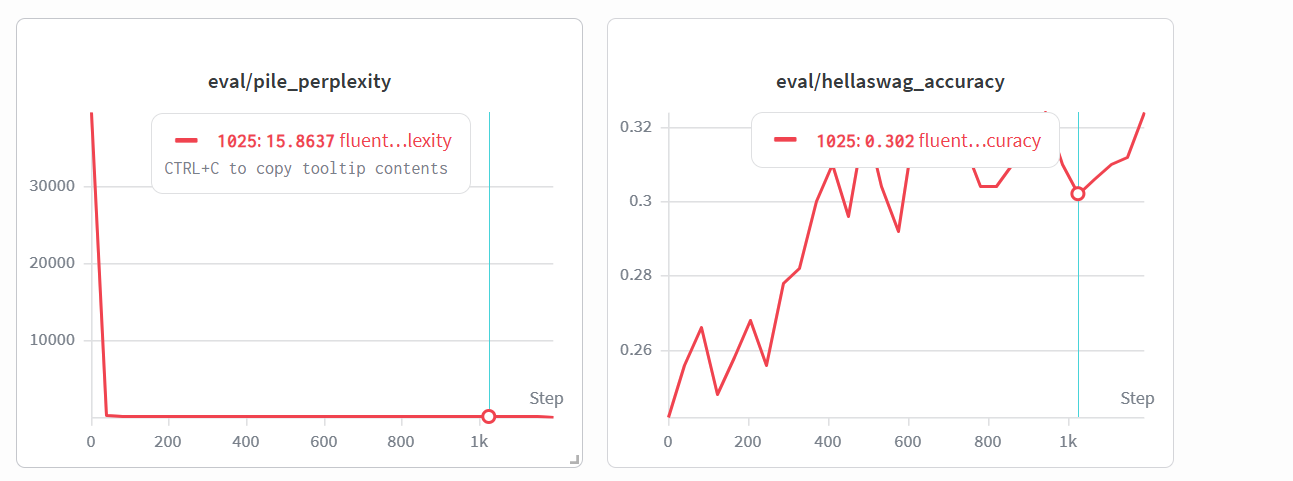
\includegraphics[width=0.95\linewidth]{Figures/tokenformer_perplexity_hellaswag_1025.png}
%         \caption{Tokenformer}
%         \label{fig:eval_tokenformer}
%     \end{subfigure}
%     \begin{subfigure}{0.9\textwidth}
%         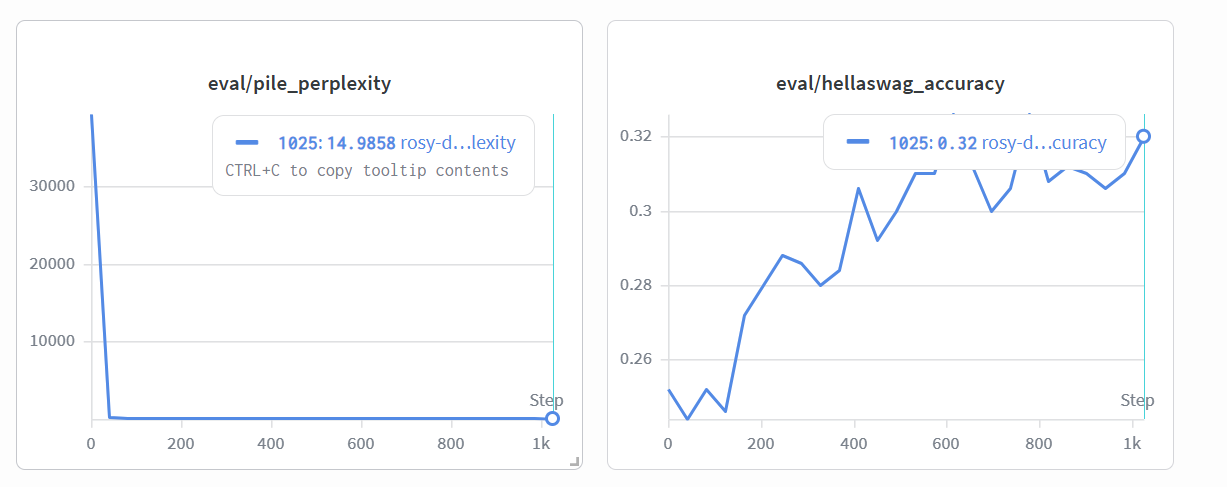
\includegraphics[width=0.95\linewidth]{Figures/tokenformer_moe_perplexity_hellaswag_1025.png}
%         \caption{Tokenformer + MoE}
%         \label{fig:eval_tokenformer_moe}
%     \end{subfigure} 
% \caption{Main plots}
% \label{fig:plots}
        
% \end{figure}


\end{document}
